\documentclass{article}
\usepackage{amsmath}
\usepackage{amssymb}
\usepackage{graphicx}
\usepackage{tikz}
\usepackage{pgfplots}
\usepackage{float}
\usepackage{subcaption}
\usepackage{geometry}

\geometry{a4paper, margin=1in}

% Define example environment
\newenvironment{example}[1]{
    \begin{trivlist}
    \item[\textbf{Example:}] #1
    \vspace{0.5em}
}{
    \end{trivlist}
    \vspace{1em}
}

\pgfplotsset{compat=1.18}
\usetikzlibrary{patterns,decorations.pathreplacing}

\title{Lecture 4 Examples}
\author{Signals and Systems Course}
\date{}

\begin{document}

\maketitle

\begin{example}[1. Discrete-Time Convolution: Exponential and Unit Step]
\textbf{Problem:}
Find the convolution $y[n] = x[n] * h[n]$ where:
\begin{align}
    x[n] &= a^n u[n], \quad |a| < 1 \\
    h[n] &= u[n]
\end{align}

\begin{figure}[H]
	\centering
	\begin{minipage}{0.45\textwidth}
		\centering
		% Scale to a fixed height of 5cm, width is automatic
		\resizebox{!}{5cm}{\begin{tikzpicture}
	\begin{axis}[
		width=12cm,
		height=7cm,
		title={Exponential Signal $x(\tau) = A e^{-a\tau}u(\tau)$},
		xlabel={$\tau$},
		ylabel={$x(\tau)$},
		axis lines=middle,
		xmin=-1, xmax=4,
		ymin=0, ymax=2.2,
		xtick=\empty, ytick=\empty,
		extra x ticks={0.333},
		extra x tick labels={$\frac{1}{a}$},
		extra y ticks={0.736, 2},
		extra y tick labels={$Ae^{-1}$, $A$},
		grid=major,
		grid style={line width=.1pt, draw=gray!30},
		]
		\addplot[blue, very thick, domain=0:4, samples=200, no marks] {2*exp(-3*x)};
		\draw[blue, very thick] (axis cs:-1,0) -- (axis cs:0,0);
		\draw[dashed, gray] (axis cs:0.333,0) -- (axis cs:0.333, {2*exp(-1)});
		\draw[dashed, gray] (axis cs:0, {2*exp(-1)}) -- (axis cs:0.333, {2*exp(-1)});
	\end{axis}
\end{tikzpicture}}
		\caption{Input signal $x[n] = a^n u[n]$}
	\end{minipage}\hfill
	\begin{minipage}{0.45\textwidth}
		\centering
		% Scale to the SAME fixed height
		\resizebox{!}{5cm}{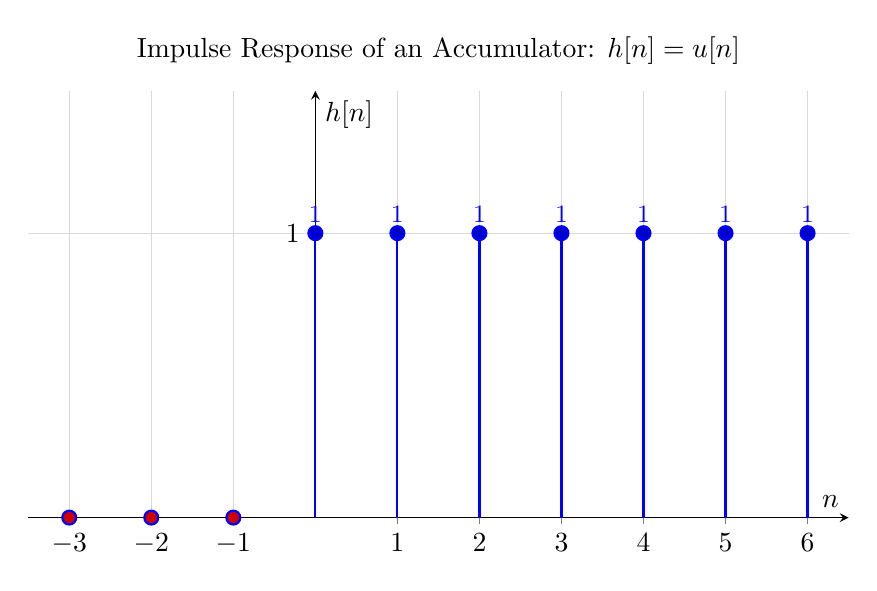
\begin{tikzpicture}
	% Define a style for our stem plots to avoid repetition
	\pgfplotsset{
		impulse/.style={
			ycomb,          % Use the 'ycomb' style for stems
			blue,           % Color of the stems and markers
			thick,          % Thickness of the stems
			mark=*,          % Marker style at the tip of the stem
			mark size=2.5pt,  % Size of the marker
		}
	}
	
	\begin{axis}[
		% Set the overall style
		width=12cm,
		height=7cm,
		% Title with context
		title={Impulse Response of an Accumulator: $h[n] = u[n]$},
		% Axis labels
		xlabel={$n$},
		ylabel={$h[n]$},
		% Position axes at the origin
		axis lines=middle,
		% Set axis limits
		xmin=-3.5, xmax=6.5,
		ymin=0, ymax=1.5,
		% Set ticks at key points
		xtick={-3, -2, -1, 0, 1, 2, 3, 4, 5, 6},
		ytick={1},
		% Add a grid
		grid=major,
		grid style={line width=.1pt, draw=gray!30},
		]
		
		% Plot the non-zero impulses and add labels above them
		\addplot+[
		impulse,
		nodes near coords={1}, % Add a '1' label to each point
		every node near coord/.style={anchor=south, font=\small}, % Position labels above
		] coordinates {
			(0, 1) (1, 1) (2, 1) (3, 1) (4, 1) (5, 1) (6, 1)
		};
		
		% Plot some zero-value points to show the effect of u[n]
		\addplot+[impulse] coordinates {
			(-3, 0)
			(-2, 0)
			(-1, 0)
		};
		
	\end{axis}
\end{tikzpicture}}
		\caption{Impulse response $h[n] = u[n]$}
	\end{minipage}
\end{figure}
\textbf{Solution:}

$$y[n] = \sum_{k=-\infty}^{\infty} x[k] h[n-k] = \sum_{k=0}^{n} a^k = \frac{1 - a^{n+1}}{1 - a}$$

For $n < 0$: $y[n] = 0$

\textbf{Answer:}
$$y[n] = \frac{1 - a^{n+1}}{1 - a} u[n]$$

\begin{figure}[H]
    \centering
    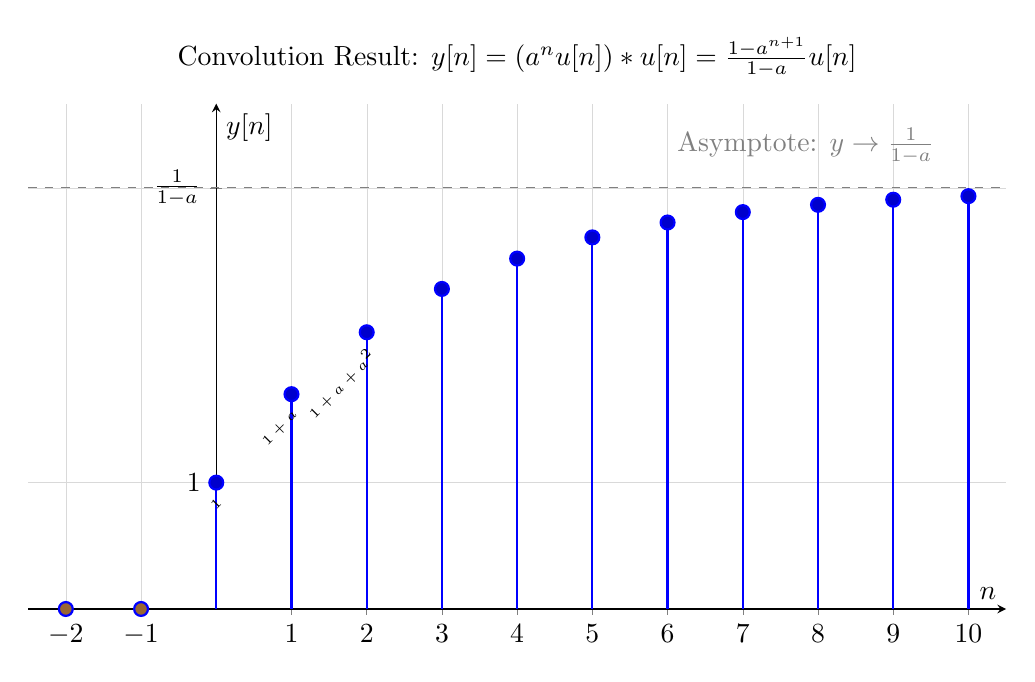
\begin{tikzpicture}
	% Define a style for stem plots
	\pgfplotsset{
		impulse/.style={
			ycomb,
			blue,
			thick,
			mark=*,
			mark size=2.5pt
		}
	}
	
	\begin{axis}[
		width=14cm,
		height=8cm,
		title={Convolution Result: $y[n] = (a^n u[n]) * u[n] = \frac{1-a^{n+1}}{1-a}u[n]$},
		xlabel={$n$},
		ylabel={$y[n]$},
		axis lines=middle,
		xmin=-2.5, xmax=10.5,
		ymin=0, ymax=4,
		xtick={-2,-1,0,1,2,3,4,5,6,7,8,9,10},
		ytick={1,10/3},
		yticklabels={$1$, $\frac{1}{1-a}$},
		grid=major,
		grid style={line width=.1pt, draw=gray!30},
		clip=false,
		]
		
		% Stem plot with custom labels (a = 0.7)
		\addplot+[
		impulse,
		nodes near coords,
		point meta=explicit symbolic,
		every node near coord/.style={
			anchor=north east,
			font=\tiny,
			rotate=45,
			text=black,
		},
		] table [meta=label] {
			x   y         label
			0   1         {$1$}
			1   1.7       {$1+a$}
			2   2.19      {$1+a+a^2$}
			3   2.533     {}
			4   2.7731    {}
			5   2.94117   {}
			6   3.058819  {}
			7   3.1411733 {}
			8   3.1988213 {}
			9   3.2391749 {}
			10  3.2674224 {}
		};
		
		% Horizontal asymptote at y = 1/(1-a) with a=0.7 -> 10/3
		\addplot[dashed, gray, samples=2] coordinates {(-2.5,10/3) (10.5,10/3)};
		\node[anchor=west, gray] at (axis cs:6,11/3) {Asymptote: $y \to \frac{1}{1-a}$};
		
		% Zero-value points to the left
		\addplot+[impulse] coordinates {(-2,0) (-1,0)};
		
	\end{axis}
\end{tikzpicture}

    \caption{Result of convolution $y[n] = x[n] * h[n]$}
\end{figure}
\end{example}

\vspace{0.5em}
\hrule
\vspace{0.5em}

\begin{example}[2. Convolution of Two Exponential Sequences]
\textbf{Problem:}
Find the convolution $y[n] = x[n] * h[n]$ where:
\begin{align}
    x[n] &= a^n u[n], \quad |a| < 1 \\
    h[n] &= b^n u[n], \quad |b| < 1
\end{align}

\textbf{Solution:}

$$y[n] = \sum_{k=0}^{n} a^k b^{n-k} = b^n \sum_{k=0}^{n} \left(\frac{a}{b}\right)^k$$

\textbf{Case 1:} $a \neq b$
$$y[n] = b^n \frac{1 - \left(\frac{a}{b}\right)^{n+1}}{1 - \frac{a}{b}} = \frac{b^{n+1} - a^{n+1}}{b - a}$$

\textbf{Case 2:} $a = b$
$$y[n] = a^n (n + 1)$$

\textbf{Answer:}
$$y[n] = \begin{cases}
    \frac{b^{n+1} - a^{n+1}}{b - a} u[n] & \text{if } a \neq b \\
    a^n (n + 1) u[n] & \text{if } a = b
\end{cases}$$
\end{example}

\vspace{0.5em}
\hrule
\vspace{0.5em}

\begin{example}[3. Convolution of Right-Sided and Left-Sided Signals]
\textbf{Problem:}
Find the convolution $y[n] = x[n] * h[n]$ where:
\begin{align}
    x[n] &= u[n] \\
    h[n] &= \left(\frac{1}{2}\right)^n u[n]
\end{align}

\textbf{Solution:}

$$y[n] = \sum_{k=0}^{n} \left(\frac{1}{2}\right)^{n-k} = \left(\frac{1}{2}\right)^n \sum_{k=0}^{n} 2^k = \left(\frac{1}{2}\right)^n \frac{2^{n+1} - 1}{2 - 1} = 2 - 2^{-n}$$

For $n < 0$: $y[n] = 0$

\textbf{Answer:}
$$y[n] = (2 - 2^{-n}) u[n]$$
\end{example}

\vspace{0.5em}
\hrule
\vspace{0.5em}

\begin{example}[4. Finite-Duration Convolution]
\textbf{Problem:}
Find the convolution $y[n] = x[n] * h[n]$ where:
\begin{align}
    x[n] &= \begin{cases}
        1 & \text{for } 0 \leq n \leq 2 \\
        0 & \text{otherwise}
    \end{cases} \\
    h[n] &= \begin{cases}
        n & \text{for } 0 \leq n \leq 2 \\
        0 & \text{otherwise}
    \end{cases}
\end{align}

\begin{figure}[H]
	\centering
	\begin{minipage}{0.45\textwidth}
		\centering
		% Scale to a fixed height, width will adjust automatically
		\resizebox{!}{5cm}{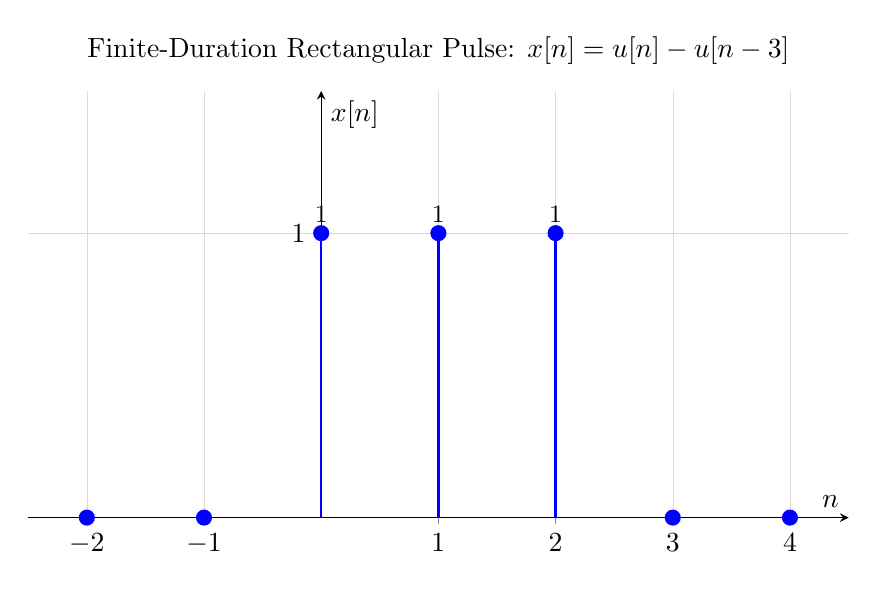
\begin{tikzpicture}
	% Define a style for our stem plots to avoid repetition
	\pgfplotsset{
		impulse/.style={
			ycomb,          % Use the 'ycomb' style for stems
			thick,          % Thickness of the stems
			mark=*,         % Marker style at the tip of the stem
			mark size=2.5pt,% Size of the marker
			blue,           % Ensure the line color is blue
			mark options={fill=blue, draw=blue}, % Explicitly set marker colors
		}
	}
	
	\begin{axis}[
		% Set the overall style
		width=12cm,
		height=7cm,
		% Title with the signal's formal definition
		title={Finite-Duration Rectangular Pulse: $x[n] = u[n] - u[n-3]$},
		% Axis labels
		xlabel={$n$},
		ylabel={$x[n]$},
		% Position axes at the origin
		axis lines=middle,
		% Set axis limits
		xmin=-2.5, xmax=4.5,
		ymin=0, ymax=1.5,
		% Set ticks at key points
		xtick={-2, -1, 0, 1, 2, 3, 4},
		ytick={1},
		yticklabels={$1$}, % Use symbolic label 'A'
		% Add a grid
		grid=major,
		grid style={line width=.1pt, draw=gray!30},
		]
		
		% Plot the non-zero impulses and add symbolic labels above them
		\addplot[
		impulse,
		nodes near coords={1}, % Display the symbol 'A' at each point
		every node near coord/.style={anchor=south, font=\small, text=black}, % Position labels
		] coordinates {
			(0, 1)
			(1, 1)
			(2, 1)
		};
		
		% Plot some zero-value points to show the signal's extent
		\addplot[impulse] coordinates {
			(-2, 0)
			(-1, 0)
			(3, 0)
			(4, 0)
		};
		
	\end{axis}
\end{tikzpicture}}
		\caption{Input signal $x[n]$}
	\end{minipage}\hfill
	\begin{minipage}{0.45\textwidth}
		\centering
		% Scale to the SAME fixed height
		\resizebox{!}{5cm}{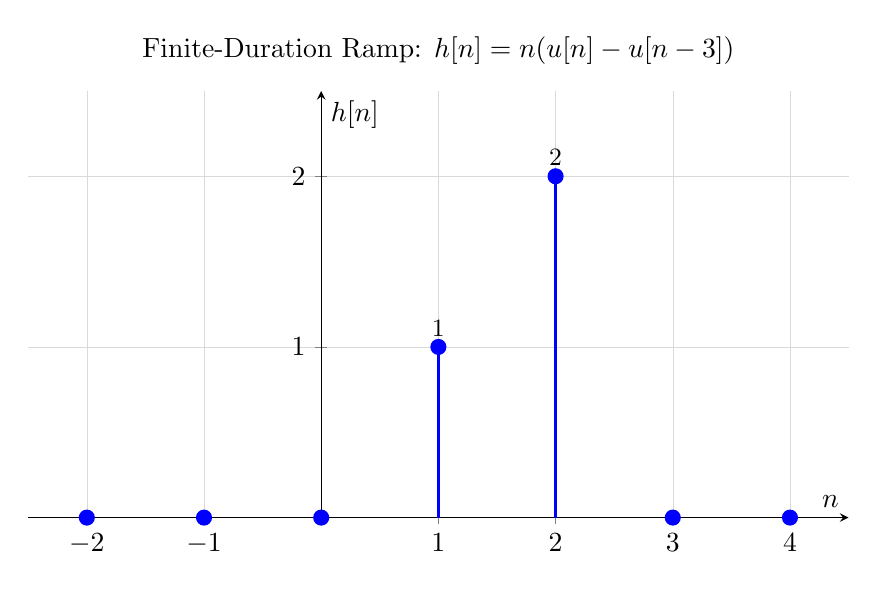
\begin{tikzpicture}
	% Define a style for our stem plots to avoid repetition
	\pgfplotsset{
		impulse/.style={
			ycomb,          % Use the 'ycomb' style for stems
			thick,          % Thickness of the stems
			mark=*,         % Marker style at the tip of the stem
			mark size=2.5pt,% Size of the marker
			blue,           % Ensure the line color is blue
			mark options={fill=blue, draw=blue}, % Explicitly set marker colors
		}
	}
	
	\begin{axis}[
		% Set the overall style
		width=12cm,
		height=7cm,
		% Title with the signal's formal definition
		title={Finite-Duration Ramp: $h[n] = n(u[n] - u[n-3])$},
		% Axis labels
		xlabel={$n$},
		ylabel={$h[n]$},
		% Position axes at the origin
		axis lines=middle,
		% Set axis limits
		xmin=-2.5, xmax=4.5,
		ymin=0, ymax=2.5,
		% Set ticks at key points
		xtick={-2, -1, 0, 1, 2, 3, 4},
		ytick={1, 2},
		% Add a grid
		grid=major,
		grid style={line width=.1pt, draw=gray!30},
		]
		
		% Plot the non-zero impulses and add value labels above them
		\addplot[
		impulse,
		nodes near coords, % Display the y-value at each point
		every node near coord/.style={anchor=south, font=\small, text=black}, % Position labels
		] coordinates {
			(1, 1)
			(2, 2)
		};
		
		% Plot the zero-value points to show the signal's extent
		\addplot[impulse] coordinates {
			(-2, 0)
			(-1, 0)
			(0, 0)
			(3, 0)
			(4, 0)
		};
		
	\end{axis}
\end{tikzpicture}}
		\caption{Impulse response $h[n]$}
	\end{minipage}
\end{figure}
\textbf{Solution:}

For each $n$, sum over the overlap region $\max(0, n-2) \leq k \leq \min(2, n)$:

\begin{align}
y[0] &= 0 \\
y[1] &= 1 \cdot 1 = 1 \\
y[2] &= 1 \cdot 2 + 1 \cdot 1 + 1 \cdot 0 = 3 \\
y[3] &= 1 \cdot 2 + 1 \cdot 1 = 3 \\
y[4] &= 1 \cdot 2 = 2
\end{align}

\textbf{Answer:}
$$y[n] = \begin{cases}
    0 & \text{for } n < 0 \text{ or } n > 4 \\
    1 & \text{for } n = 1 \\
    3 & \text{for } n = 2, 3 \\
    2 & \text{for } n = 4
\end{cases}$$

\begin{figure}[H]
    \centering
    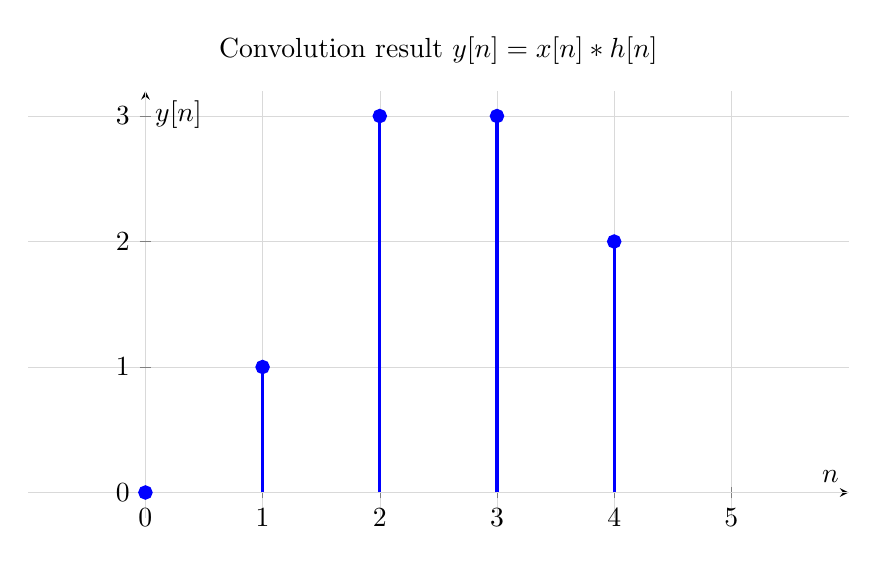
\begin{tikzpicture}
\begin{axis}[
    width=12cm,
    height=7cm,
    axis lines=middle,
    xlabel={$n$},
    ylabel={$y[n]$},
    title={Convolution result $y[n] = x[n] * h[n]$},
    xmin=-1, xmax=6,
    ymin=-0.2, ymax=3.2,
    xtick=\empty,
    ytick=\empty,
    extra x ticks={0, 1, 2, 3, 4, 5},
    extra y ticks={0, 1, 2, 3},
    grid=major,
    grid style={line width=.1pt, draw=gray!30},
]

% Plot the convolution result
\addplot[ycomb, blue, very thick, mark=*, mark size=2pt] coordinates {(0,0) (1,1) (2,3) (3,3) (4,2)};

\end{axis}
\end{tikzpicture}


    \caption{Result of convolution $y[n] = x[n] * h[n]$}
\end{figure}
\end{example}

\vspace{0.5em}
\hrule
\vspace{0.5em}

\begin{example}[5. Convolution of Two Finite-Length Sequences]
\textbf{Problem:}
Find $y[n] = x[n] * h[n]$ where:
\[ h[n] = \begin{cases} 1 & n=0 \\ -1/2 & n=1 \\ 0 & \text{otherwise} \end{cases} \]
\[ x[n] = \begin{cases} 1 & n=-1 \\ 2 & n=0 \\ -1 & n=1 \\ 0 & \text{otherwise} \end{cases} \]

\begin{figure}[H]
    \centering
    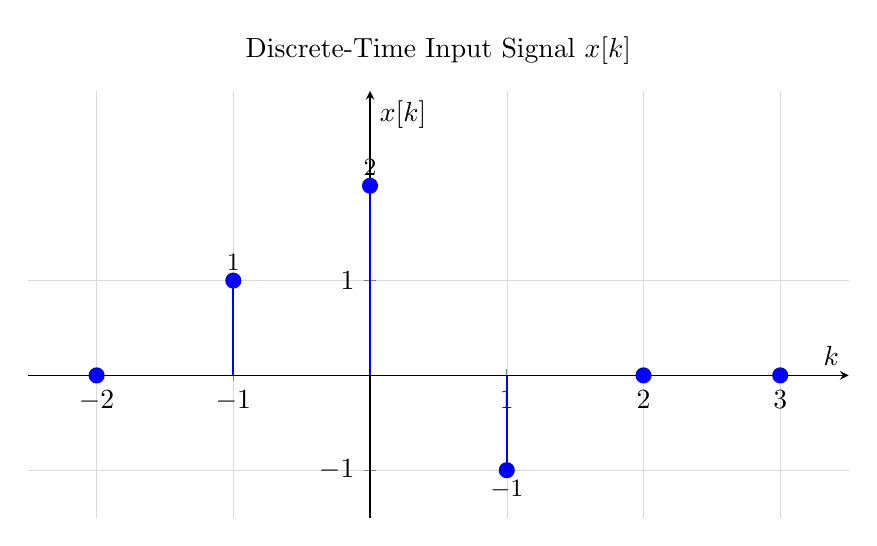
\begin{tikzpicture}
	% Define a style for our stem plots
	\pgfplotsset{
		impulse/.style={
			ycomb,
			blue,
			thick,
			mark=*,
			mark size=2.5pt,
			mark options={fill=blue, draw=blue},
		}
	}
	
	\begin{axis}[
		width=12cm,
		height=7cm,
		title={Discrete-Time Input Signal $x[k]$},
		xlabel={$k$},
		ylabel={$x[k]$},
		axis lines=middle,
		xmin=-2.5, xmax=3.5,
		ymin=-1.5, ymax=3,
		xtick={-2, -1, 0, 1, 2, 3},
		ytick={-1, 1},
		grid=major,
		grid style={line width=.1pt, draw=gray!30},
		]
		
		% Plot positive values with labels above
		\addplot[
		impulse,
		nodes near coords,
		every node near coord/.style={anchor=south, font=\small, text=black},
		] coordinates {(-1,1) (0,2)};
		
		% Plot negative values with labels below
		\addplot[
		impulse,
		nodes near coords,
		every node near coord/.style={anchor=north, font=\small, text=black},
		] coordinates {(1,-1)};
		
		% Plot zero-value points
		\addplot[impulse] coordinates {(-2,0) (2,0) (3,0)};
		
	\end{axis}
\end{tikzpicture}
    \caption{The finite-length input signal $x[k]$.}
\end{figure}

\textbf{Solution:}
$y[n]$ is non-zero for $n \in \{-1, 0, 1, 2\}$:

\begin{align}
y[-1] &= x[-1]h[0] = (1)(1) = 1 \\
y[0] &= x[-1]h[1] + x[0]h[0] = (1)(-1/2) + (2)(1) = 3/2 \\
y[1] &= x[0]h[1] + x[1]h[0] = (2)(-1/2) + (-1)(1) = -2 \\
y[2] &= x[1]h[1] = (-1)(-1/2) = 1/2
\end{align}

\textbf{Alternative:} Decompose $x[n] = \delta[n+1] + 2\delta[n] - \delta[n-1]$
Then $y[n] = h[n+1] + 2h[n] - h[n-1]$ gives same result.

\begin{figure}[H]
    \centering
    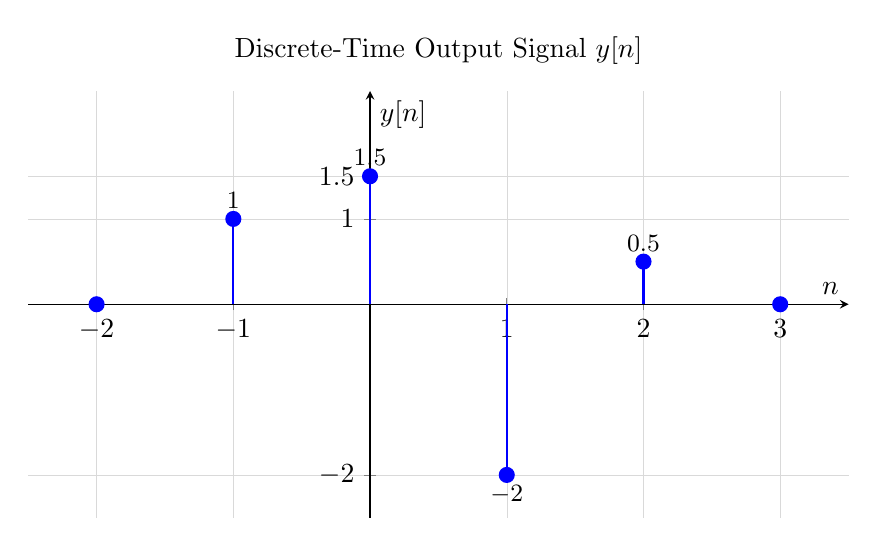
\begin{tikzpicture}
	% Define a style for our stem plots
	\pgfplotsset{
		impulse/.style={
			ycomb,
			blue,
			thick,
			mark=*,
			mark size=2.5pt,
			mark options={fill=blue, draw=blue},
		}
	}
	
	\begin{axis}[
		width=12cm,
		height=7cm,
		title={Discrete-Time Output Signal $y[n]$},
		xlabel={$n$},
		ylabel={$y[n]$},
		axis lines=middle,
		xmin=-2.5, xmax=3.5,
		ymin=-2.5, ymax=2.5,
		xtick={-2, -1, 0, 1, 2, 3},
		ytick={-2, 1, 1.5},
		grid=major,
		grid style={line width=.1pt, draw=gray!30},
		]
		
		% Plot positive values with labels above
		\addplot[
		impulse,
		nodes near coords,
		every node near coord/.style={anchor=south, font=\small, text=black},
		] coordinates {(-1,1) (0,1.5) (2,0.5)};
		
		% Plot negative values with labels below
		\addplot[
		impulse,
		nodes near coords,
		every node near coord/.style={anchor=north, font=\small, text=black},
		] coordinates {(1,-2)};
		
		% Plot zero-value points
		\addplot[impulse] coordinates {(-2,0) (3,0)};
		
	\end{axis}
\end{tikzpicture}
    \caption{The final output signal $y[n]$.}
\end{figure}

\textbf{Answer:} $y[n] = \{1, 3/2, -2, 1/2\}$ for $n = \{-1, 0, 1, 2\}$, 0 otherwise
\end{example}

\end{document}